\section{Design a Neural Network}
Design a Neural network capable of generating Hamming codes for 4-bit inputs. Describe the network, including the number of neurons in each layer and determine all the weights in the network. (note that the neural net should have 4 inputs and 3 outputs.)
\begin{qsolve}
    \begin{qsolve}[]
        the inputs to the network are the 4 bits of the input, and the outputs are the 3 parity bits.
        $$P_1 = d_2 \oplus d_3 \oplus d_4$$
        $$P_2 = d_1 \oplus d_3 \oplus d_4$$
        $$P_3 = d_1 \oplus d_2 \oplus d_4$$
        \begin{center}
            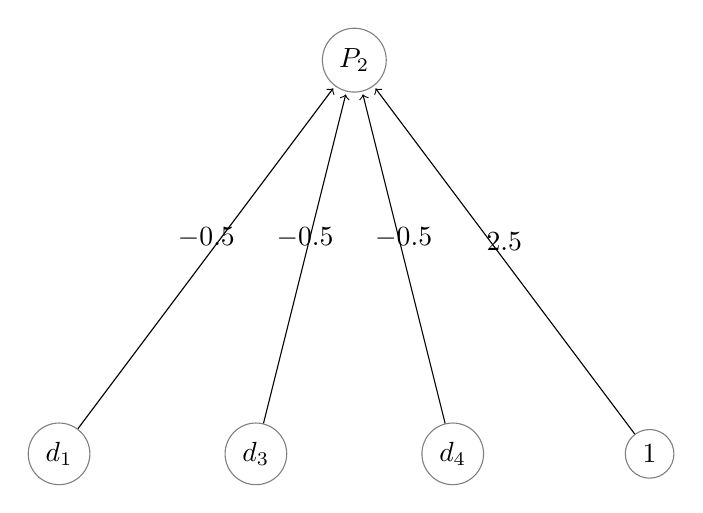
\begin{tikzpicture}[shorten >=1pt,->,draw=black!50, node distance=2cm]
                % Nodes
                \node[circle, draw] (P2) at (3.75, 0) {$P_2$};
                \node[circle, draw] (d1) at (0, -5) {$d_1$};
                \node[circle, draw] (d3) at (2.5, -5) {$d_3$};
                \node[circle, draw] (d4) at (5, -5) {$d_4$};
                \node[circle, draw] (b) at (7.5, -5) {$1$};
                % Edges
                \draw[->, black] (d1) -- node[above] {$-0.5$} (P2);
                \draw[->, black] (d3) -- node[above] {$-0.5$} (P2);
            
                \draw[->, black] (d4) -- node[above] {$-0.5$} (P2);
            
                \draw[->, black] (b) -- node[above] {$2.5$} (P2);
                
            \end{tikzpicture}
        \end{center}
        the network for $P_2$ can be design as the above figure. for $P_1$ and $P_3$ the network can be designed similarly. the activation function for the neurons is the step function. in total we have 4 neurons in the input layer, 3 neurons in the output layer, and 12 neurons in the hidden layer. the weights are as follows:
        $$W_1 = \begin{bmatrix}
            1 & 1 & -1 & -1\\
            1 & -1 & 1 & -1\\
            0 & 0 & 0 & 0\\
            1 & -1 & -1 & 1\\
        \end{bmatrix}$$
        \splitqsolve[\splitqsolve]
        $$W_2 = \begin{bmatrix}
            1 & 1 & -1 & -1\\
            0 & 0 & 0 & 0\\
            1 & -1 & 1 & -1\\
            1 & -1 & -1 & 1\\
        \end{bmatrix}$$
        $$W_3 = \begin{bmatrix}
            0 & 0 & 0 & 0\\
            1 & 1 & -1 & -1\\
            1 & -1 & 1 & -1\\
            1 & -1 & -1 & 1\\
        \end{bmatrix}$$
        so we have:
        $$W = \begin{bmatrix}
            W_1 & W_2 & W_3
        \end{bmatrix}$$
        

        
    \end{qsolve}
\end{qsolve}